%TCIDATA{LaTeXparent=0,0,relatorio.tex}
\ifx\compilewholereport\undefined
	\documentclass[11pt,a4paper,oneside]{book}
	
	% Escolher um dos seguintes formatos:
	\usepackage{ft2unb} % segue padrão de fontes do Latex
	
	% Pacotes
	\usepackage{graphicx}
	\usepackage{amsfonts}
	\usepackage{amsmath}
	\usepackage{amssymb}
	\usepackage[thmmarks,amsmath]{ntheorem}
	\usepackage{boxedminipage}
	\usepackage{theorem}
	\usepackage{fancybox}
	\usepackage{fancyhdr}
	\usepackage{url}
	\usepackage{afterpage}
	\usepackage{color}
	\usepackage{colortbl}
	\usepackage{rotating}
	\usepackage{makeidx}
	\usepackage{indentfirst}
	\usepackage{bibentry}
	\usepackage{subcaption}
	\usepackage{todonotes}
	\presetkeys{todonotes}{inline}{}
	
	\begin{document}
	\frontmatter
	\listoftodos
	\mainmatter
	
	%%%%%%%%%%%%%%%%%%%%%%%%%%%%
	%%%%%%%% Apagar coisas acima
	%%%%%%%%%%%%%%%%%%%%%%%%%%%%
\fi
                      
\chapter{Desenvolvimento}\label{CapDesenvolvimento}

\resumodocapitulo{Este capítulo trata da concepção dos experimentos realizados. Nele serão descritos com detalhes cada um dos experimentos, ficando a parte de análise reservada ao capítulo \ref{CapExperimentos}.}

\section{Introdu\c{c}\~{a}o}
%\vspace{0.8cm}
Devido ao caráter experimental e exploratório do objetivo proposto na seção \ref{sec:projeto}, decidiu-se dividir o projeto em vários experimentos menores.
Desta forma, além de garantir algum material mesmo que tudo dê errado, consegue-se simplificar o processo de pesquisa e desenvolvimento através dos pequenos passos e análises frequentes.

Como o objetivo final do projeto é a familiarização com as ferramentas e processos envolvidos na autoreconfiguração, decidiu-se começar estudando os elementos necessários para se realizar a reconfiguração dinâmica.
O passo seguinte mais lógico é o de estudar como funciona as memórias dos sistema.
Em seguida, o estudo da inicialização da memória se faz muito importante.
O último passo seria entender como funciona a autoreconfiguração em baixo nível, ou seja, como os dados devem ser entregues aos devidos componentes para que ela aconteça.

\begin{figure}[h]
\centering
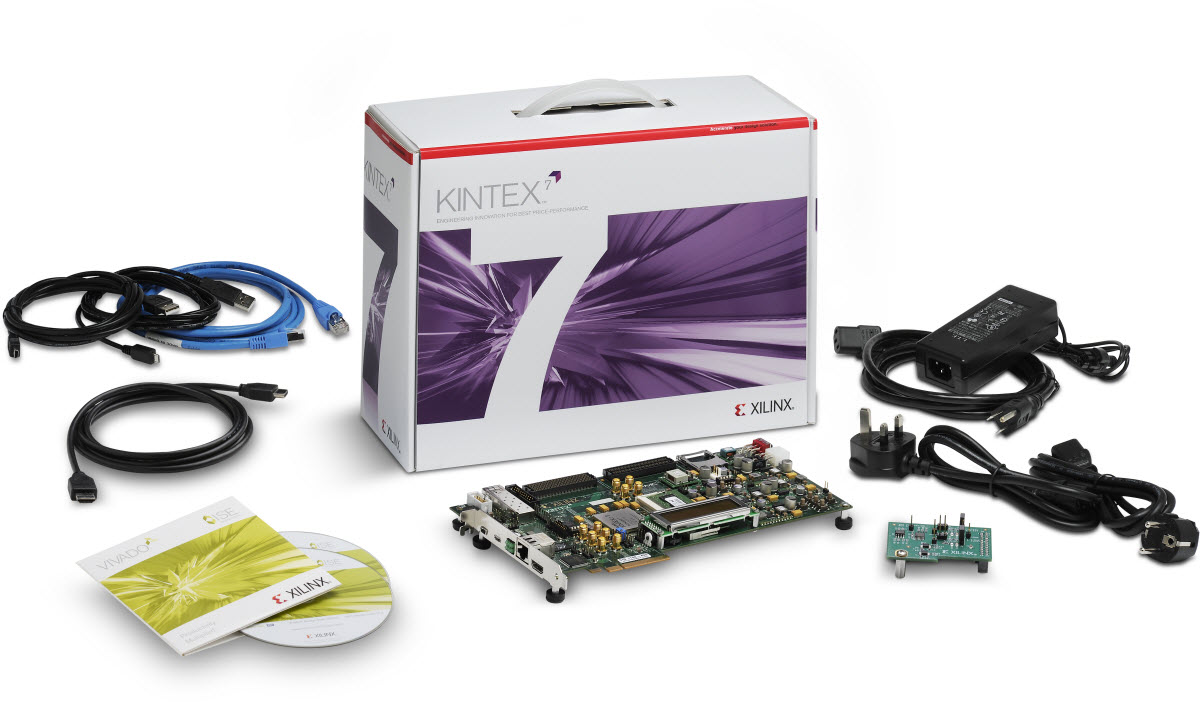
\includegraphics[width=0.5\textwidth]{figs/kintex-7_kc705}
\caption{Foto ilustrativa do kit de desenvolvimento Kintex-7 KC705 extraida do site da Xilinx.}
\label{fig:kressarray}
\end{figure}

Para o desenvolvimento desse projeto, escolheu-se, por motivos arbitrários, utilizar o kit de desenvolvimento da Xilinx\textregistered{} chamado Kintex-7 KC705.
O único critério foi a disponibilidade dos equipamentos no início do projeto e a capacidade do dispositivo de fazer o que deseja-se.
Este kit possui FPGA modelo XC7K325T-2FFG900C, leitor de cartão de memória, conector PCIe\textregistered{}, memória DDR3, visor de 7-segmentos, porta ethernet e dentre outras coisas.

\section{Experimento 1 - Teste da Reconfiguração Dinâmica}
\todo{Descrever o experimento 1}
\todo{Explicar como fui para o próximo experimento}
\section{Experimento 2 - Teste de Acesso a Memória}
\todo{Descrever o experimento 2}
\todo{Descrever os tipos de memória disponíveis e o porque de escolher a DDR3}
\todo{Explicar porque não deu certo e como fui para o próximo experimento}
\section{Experimento 3 - Teste do \textit{Bootloader}}
\todo{Descrever o experimento 3}
\todo{Explicar como fui para o próximo experimento}
\section{Experimento 4 - Teste da Autoreconfiguração com \textit{Bootloader} Dedicado}
\todo{Descrever o experimento 4}
\todo{Explicar como fui para o próximo experimento}
\section{Experimento 5 - Teste da Autoreconfiguração}
\todo{Descrever o experimento 5}
\todo{Explicar como fui para o próximo experimento}

\ifx\compilewholereport\undefined
	\bibliographystyle{authordate1} 
	%\bibliography{bibliografia}
	\newsavebox\mytempbib\savebox\mytempbib{\parbox{\textwidth}{\bibliography{bibliografia}}}

	\end{document}
\fi